\documentclass[a4paper,14pt]{extarticle}

% Путь до папки с общими шаблонами
\newcommand{\pathToCommonFolder}{/home/denilai/Documents/repos/latex/Common}
% Название работы в титуле
\newcommand{\workname}{Отчет по практической работе №4}
% Название дисциплины в титуле
\newcommand{\discipline}{Архитектура процессоров и микропроцессоров}
% Название кафедры в титуле
\newcommand{\kafedra}{Кафедра вычислительной техники}
% Тема работы в титуле
\newcommand{\theme}{Стадии выполнения команд процессором КР580ВМ80}
% Должность преподавателя в титуле
\newcommand{\rang}{cтарший преподаватель кафедры ВТ}
% ФИО преподавателя в титуле
\newcommand{\teacherfio}{Ю.~М.Скрябин}
\newcommand{\studentfio}{А.~М.~Сосунов}%Д.~Н.~Федосеев\\%А.~М.~Сосунов\\%К.~Ю.~Денисов\\
\newcommand{\signature}{\pathToCommonFolder/sosunov-signature}
\def\myformat#1{\hfil #1\hfil}


\newcommand{\heading}[1]{\multicolumn{1}{|c|}{#1}}

% установка размера шрифта для всего документа
%\fontsize{20pt}{18pt}\selectfont
\usepackage{extsizes} % Возможность сделать 14-й шрифт

% Вставка заготовки преамбулы
% Этот шаблон документа разработан в 2014 году
% Данилом Фёдоровых (danil@fedorovykh.ru) 
% для использования в курсе 
% <<Документы и презентации в \LaTeX>>, записанном НИУ ВШЭ
% для Coursera.org: http://coursera.org/course/latex .
% Исходная версия шаблона --- 
% https://www.writelatex.com/coursera/latex/5.3

% В этом документе преамбула

% Для корректного использования русских символов в формулах
% пакеты hyperref и настройки, связанные с ним, стоит загуржать
% перед загрузкой пакета mathtext



% поддержка русских букв
% кодировка шрифта
%\usepackage[T2A]{fontenc} 
\usepackage{pscyr}

% использование ненумеровонного абзаца с добавлением его в содержаниеl

\newcommand{\anonsection}[1]{\section*{#1}\addcontentsline{toc}{section}{#1}}
\newcommand{\sectionunderl}[1]{\section*{\underline{#1}}}


% настройка окружения enumerate
\usepackage{enumitem}
\setlist{noitemsep}
\setlist[enumerate]{labelsep=*, leftmargin=1.5pc}

\usepackage{hyperref}

% сначала ставить \usepackage{extsizes} % Возможность сделать 14-й шрифт
% для корректной установки полей вставлять преамбулу следует в последнюю очередь (но перед дерективой замены \rmdefault)
\usepackage[top=20mm,bottom=25mm,left=35mm,right=20mm]{geometry} % Простой способ задавать поля

\hypersetup{				% Гиперссылки
	unicode=true,           % русские буквы в раздела PDF
	pdftitle={Заголовок},   % Заголовок
	pdfauthor={Автор},      % Автор
	pdfsubject={Тема},      % Тема
	pdfcreator={Создатель}, % Создатель
	pdfproducer={Производитель}, % Производитель
	pdfkeywords={keyword1} {key2} {key3}, % Ключевые слова
	colorlinks=true,       	% false: ссылки в рамках; true: цветные ссылки
	linkcolor=red,          % внутренние ссылки
	citecolor=black,        % на библиографию
	filecolor=magenta,      % на файлы
	urlcolor=blue           % на URL
}

%%% Работа с русским языком
\usepackage{cmap}					% поиск в PDF
\usepackage{mathtext} 				% русские буквы в формулах
\usepackage[T2A]{fontenc}			% кодировка
\usepackage[utf8]{inputenc}			% кодировка исходного текста
\usepackage[english,russian]{babel}	% локализация и переносы
\usepackage{indentfirst}
\frenchspacing

%для изменения названия списка иллюстраций
\usepackage{tocloft}


\renewcommand{\epsilon}{\ensuremath{\varepsilon}}
\renewcommand{\phi}{\ensuremath{\varphi}}
\renewcommand{\kappa}{\ensuremath{\varkappa}}
\renewcommand{\le}{\ensuremath{\leqslant}}
\renewcommand{\leq}{\ensuremath{\leqslant}}
\renewcommand{\ge}{\ensuremath{\geqslant}}
\renewcommand{\geq}{\ensuremath{\geqslant}}
\renewcommand{\emptyset}{\varnothing}

% Изменения параметров списка иллюстраций
\renewcommand{\cftfigfont}{Рисунок } % добавляем везде "Рисунок" перед номером
\addto\captionsrussian{\renewcommand\listfigurename{Список иллюстративного материала}}

\newcommand{\tm}{\texttrademark\ }
\newcommand{\reg}{\textregistered\ }


%%% Дополнительная работа с математикой
\usepackage{amsmath,amsfonts,amssymb,amsthm,mathtools} % AMS
\usepackage{icomma} % "Умная" запятая: $0,2$ --- число, $0, 2$ --- перечисление

%% Номера формул
%\mathtoolsset{showonlyrefs=true} % Показывать номера только у тех формул, на которые есть \eqref{} в тексте.
%\usepackage{leqno} % Нумереация формул слева

%% Свои команды
\DeclareMathOperator{\sgn}{\mathop{sgn}}

%% Перенос знаков в формулах (по Львовскому)
\newcommand*{\hm}[1]{#1\nobreak\discretionary{}
{\hbox{$\mathsurround=0pt #1$}}{}}


% отступ для первого абзаца главы или параграфа
%\usepackage{indentfirst}

%%% Работа с картинками
\usepackage{graphicx}  % Для вставки рисунков
\graphicspath{{images/}{screnshots/}}  % папки с картинками
\DeclareGraphicsExtensions{.pdf,.png,.jpg}
\setlength\fboxsep{3pt} % Отступ рамки \fbox{} от рисунка
\setlength\fboxrule{1pt} % Толщина линий рамки \fbox{}
\usepackage{wrapfig} % Обтекание рисунков текстом

%%% Работа с таблицами
\usepackage{array,tabularx,tabulary,booktabs} % Дополнительная работа с таблицами
\usepackage{longtable}  % Длинные таблицы
\usepackage{multirow} % Слияние строк в таблице

%%% Теоремы
\theoremstyle{plain} % Это стиль по умолчанию, его можно не переопределять.
\newtheorem{theorem}{Теорема}[section]
\newtheorem{proposition}[theorem]{Утверждение}

\theoremstyle{plain} % Это стиль по умолчанию, его можно не переопределять.
\newtheorem{work}{Практическая работа}[part]


 
 
\theoremstyle{definition} % "Определение"
\newtheorem{corollary}{Следствие}[theorem]
\newtheorem{problem}{Задача}[section]
 
\theoremstyle{remark} % "Примечание"
\newtheorem*{nonum}{Решение}



%%% Программирование
\usepackage{etoolbox} % логические операторы

%%% Страница

%	\usepackage{fancyhdr} % Колонтитулы
% 	\pagestyle{fancy}
%   \renewcommand{\headrulewidth}{0pt}  % Толщина линейки, отчеркивающей верхний колонтитул
% 	\lfoot{Нижний левый}
% 	\rfoot{Нижний правый}
% 	\rhead{Верхний правый}
% 	\chead{Верхний в центре}
% 	\lhead{Верхний левый}
%	\cfoot{Нижний в центре} % По умолчанию здесь номер страницы

\usepackage{setspace} % Интерлиньяж
\onehalfspacing % Интерлиньяж 1.5
%\doublespacing % Интерлиньяж 2
%\singlespacing % Интерлиньяж 1

\usepackage{lastpage} % Узнать, сколько всего страниц в документе.

\usepackage{soul} % Модификаторы начертания


\usepackage[usenames,dvipsnames,svgnames,table,rgb]{xcolor}


\usepackage{csquotes} % Еще инструменты для ссылок

%\usepackage[style=authoryear,maxcitenames=2,backend=biber,sorting=nty]{biblatex}

\usepackage{multicol} % Несколько колонок

\usepackage{tikz} % Работа с графикой
\usepackage{pgfplots}
\usepackage{pgfplotstable}

% модуль для вставки рыбы
\usepackage{blindtext}

\usepackage{listings}
\usepackage{color}


% для поворота отдельной страницы. Использовать окружение \landscape
\usepackage{pdflscape} 
\usepackage{rotating} 


\definecolor{mygreen}{rgb}{0,0.6,0}
\definecolor{mygray}{rgb}{0.5,0.5,0.5}
\definecolor{mymauve}{rgb}{0.58,0,0.82}


% пример импорта файла
%\lstinputlisting{/home/denilai/repomy/conf/distributions}

\lstset{
	language=Python,
	basicstyle=\footnotesize,        % the size of the fonts that are used for the code
	numbers=left,                    % where to put the line-numbers; possible values are (none, left, right)
	numbersep=5pt,                   % how far the line-numbers are from the code
	numberstyle=\tiny\color{mygray}, % the style that is used for the line-numbers
	stepnumber=2,                    % the step between two line-numbers. If it's 1, each line will be numbered
	% Tab - 2 пробела
	tabsize=2,    
	% Автоматический перенос строк
	breaklines=true,
	frame=single,
	breakatwhitespace=true,
	title=\lstname 
}



\author{Кирилл Денисов}
\title{Лабораторная работа №1}
\date{\today}

\renewcommand{\withouttheme}{1}

% установка полуторного интервала
% \usepackage{setspace}  
% \onehalfspacing

% использовать Times New Roman
\renewcommand{\rmdefault}{ftm}


\begin{document}
	\thispagestyle{empty}
	% Вставка первого титульного листа
	%\newcommand{\withouttheme}{} добавить эту переменную для определения, нужна ли тема
%     {} - нужна
%    {1} - не нужна

%\newcommand{\withoutsubmissiondate}{} добавить эту переменную для определения, нужен ли срок предоставления отчета
%     {} - нужен
%    {1} - не нужен
\begin{center}
	\begin{figure}[h!]
		\begin{center}
		
\includegraphics[width=0.17\linewidth]{\pathToCommonFolder/gerb}
		%\caption{}\label{pic:first}
		%	\vspace{5ex}
		\end{center}	
	\end{figure}
 	\small	МИНОБРНАУКИ РОССИИ \\
	Федеральное государственное бюджетное образовательное учреждение\\
						высшего профессионального образования\\
\normalsize					
\textbf{«МИРЭА – Российский технологический университет»\\
						РТУ МИРЭА}\\
						\noindent\rule{1\linewidth}{1pt}\\
       Институт информационных технологий\\ %\vspace{2ex}
					\kafedra\\
		\vspace{3ex}
			\large \textbf{\workname}  \\
		%\vspace{1ex}
						по дисциплине\\ «\discipline» \\
		\vspace{3ex}
		\if \withouttheme
			\textbf{Тема работы:}\\ <<\theme>>
		\fi
\vspace{3ex}
\small
\begin{table}[h!]
\begin{tabular}{p{0.14\linewidth}p{0.38\linewidth}p{0.25\linewidth}p{0.2\linewidth}}
	\textbf{Выполнил:} & студент группы ИВБО-02-19 & \studentfio &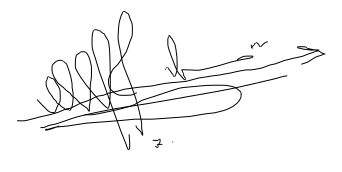
\includegraphics[width=0.8\linewidth]{\signature}\\ \\
	\textbf{Принял:} & \rang & \teacherfio 
\end{tabular}
\end{table}
\end{center}

\begin{flushleft}
	\begin{tabular}{p{0.25\linewidth}l}

		Работа выполена & <<\noindent\rule{2em}{1pt}>>
		                    \noindent\rule{5em}{1pt} 202\noindent\rule{1em}{1pt} \\

		<<Зачтено>> & <<\noindent\rule{2em}{1pt}>>
		\noindent\rule{5em}{1pt} 202\noindent\rule{1em}{1pt} \\

	\end{tabular}
\end{flushleft}

\normalsize
\begin{center}	
\vfill 
Москва 2021
\end{center}

	\newpage
	%\tableofcontents
	\newpage
	%\listoftables

	\section*{\myformat{ПЕРЕЧЕНЬ СОКРАЩЕНИЙ}}
	МКП --- микропрограмма
	
	МПА --- микропрограммный автомат
	
	УАПЛ --- управляющий автомат на программируемой логике
	
	ГСА --- граф-схема автомата
	
	АЛУ --- арифметико-логическое устройство
	
	УУ --- устройство управления
	
	КС1 --- первая комбинационная схема 
	
	КС2 --- вторая комбинационная схема 
	
	ОП --- операционное поле
	
	АП --- адресное поле 
	
	БП --- безусловный переход
	
	УП --- условный переход
	
	
	%ША --- шина адреса
	
	%ШД --- шина данных
	
	%ШУ --- шина управления
	
	СЧАМК --- счетчик адреса микрокоманд
	
	ОЗУ  --- оперативное запоминающее устройство
	
	%	$РА_{ОЗУ}$ --- регистр адреса оперативного запоминающего устройства
	
	%	$РД_{ОЗУ}$ --- регистр данных оперативного запоминающего устройства
	
	%	$ШД_{ОЗУ}$ --- шина адреса оперативного запоминающего устройства
	
	РК  --- регистр команд
	
	РС  --- распределитель сигналов
	
	DC  --- дешифратор
	
	%SM -- сумматор
	
	КОП --- код операции
	
	%РА1, РА2 --- входные регистры АЛУ
	
	%РС1, РС2 --- входные регистры сумматора
	
	%	$РР_{АЛУ}$ --- регистр результата АЛУ
	
	РОН --- регистр общего назначения
	
	%ЧТРОН --- управляющий сигнал на чтение РОН
	
	%	$РД_{РОН}$  --- регистр данных регистров общего назначения
	
	%	$РА_{РОН}$  --- регистр адреса регистров общего назначения
	
	%УС --- указатель стека
	
	
	\newpage
	\section*{Задание}
	Для заданного в таблице 4 закодированного графа разработать три микропрограммных автомата (МПА):
	\begin{enumerate}
		\item МПА Мили на жесткой логике;
		\item Управляющий автомат на программируемой
		логике (УАПЛ) с принудительной адресацией с 2-я адресными полями;
		\item УАПЛ с естественной адресацией. 
	\end{enumerate}
	Для УАПЛ выбрать смешанный способ микропрограммирования.
	
\section* {Ход работы}
	В ходе данной лабораторной работы нам было предложено разработать три микропрограммных автомата (МПА). Приведем абстрактный граф-схему автомата (ГСА) (см. Рисунок \ref{fig:gsa}). Где  $a_1 ... a_5$ --- состояния автомата, причем $a'_1$~---~конечное состояние автомата.
	% TODO: \usepackage{graphicx} required
	\begin{figure}[h!]
		\centering
		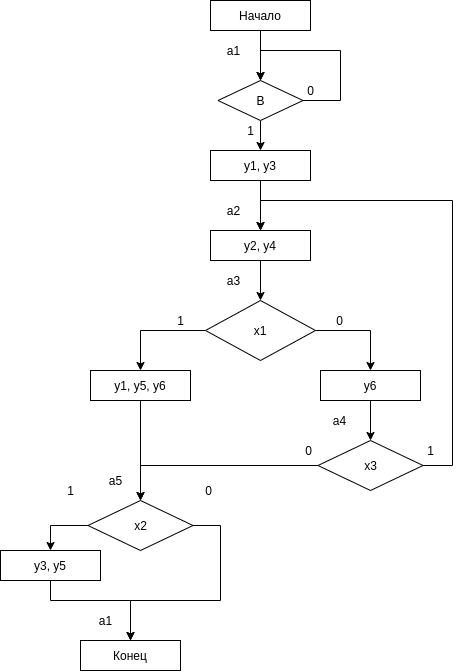
\includegraphics[width=0.5\linewidth]{gsa}
		\caption{Граф-схема автомата}
		\label{fig:gsa}
	\end{figure}
	
	Получим закодированный граф на базе ФСА, заменив микрооперации
	управляющими сигналами \{y\}, а логические условия~---~осведомительными сигналами~\{x\}.
	
	Рассмотрим реализацию блока управления на базе МПА с жесткой логикой (автомат Мили), приведенного на Рисунке \ref{fig:mili}.
	
	% TODO: \usepackage{graphicx} required
	\begin{figure}[h!]
		\centering
		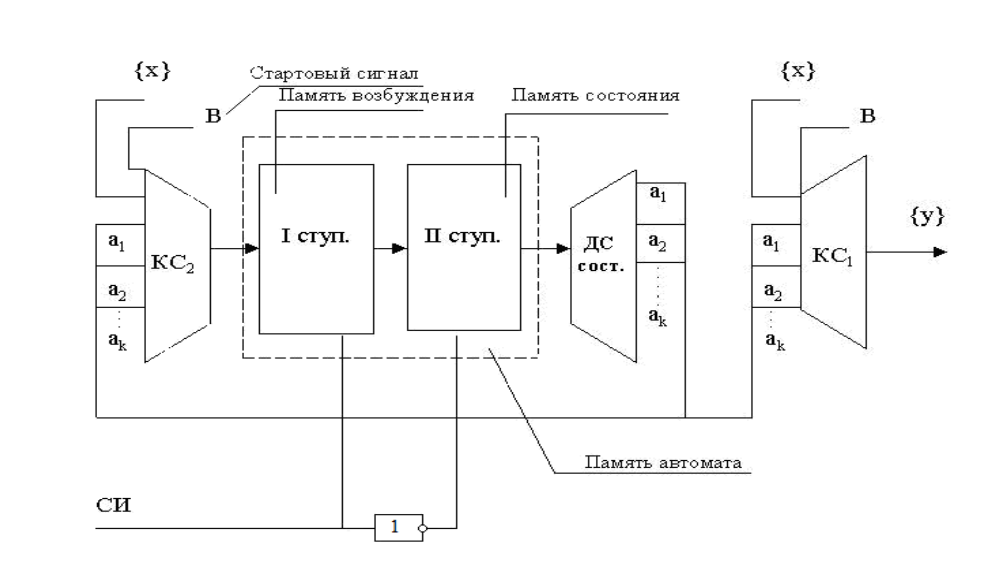
\includegraphics[width=0.8\linewidth]{mili}
		\caption{МПА на жесткой логике на базе автомата Мили }
		\label{fig:mili}
	\end{figure}
%\newpage
В состав \ref{fig:mili} МПА входят следующие структурные элементы: 
\begin{itemize}
	\item 2-х ступенчатая память автомата;
	\item дешифратор состояния (ДСсост.);
	\item две комбинационные схемы КС1 и КС2. 
\end{itemize}
Память служит для запоминания состояния автомата.

Во второй ступени фиксируется текущее состояние, по которому комбинационная
схема КС1 формирует набор управляющих сигналов. Первая ступень предназначена
для формирования следующего состояния в зависимости от предыдущего и
значений осведомительных сигналов. Переключение первой ступени памяти осуществляет схема КС1.

Двухступенчатая память применяется для исключения
<<гонок>> из-за разницы в величине задержек в КС1 при переключении различных разрядов памяти.

Для ГСА (Рисунок \ref{fig:gsa}) выходы операторных вершин, отмеченные символами $a_1 ... a_5$ соответствуют состояниям памяти МПА. Присвоим состояниям двоичные коды:
\begin{align*}
 	a1(a1') &= 000 \\
 	a2 &= 001 \\ 
 	a3 &= 010 \\
 	 a4 &= 011 \\
 	 a5 &= 100
\end{align*}


Для кодирования пяти состояний потребовалось три двоичных разряда, 
соответственно память автомата будет строиться на трех триггерах.
Выход вершины <<начало>> и вход в вершину <<конец>> отмечен одним и
тем же символом а1. Это соответствует одному и тому же состоянию памяти и
означает, что после выполнение своих функций по генерации \{y\} в соответствии заданной ГСА, МПА возвращается в исходное положение до следующей
инициализации. Для этого в ГСА после вершины <<Начало>> необходимо поставить ждущую вершину:

% TODO: \usepackage{graphicx} required
\begin{figure}[htbp]
	\centering
	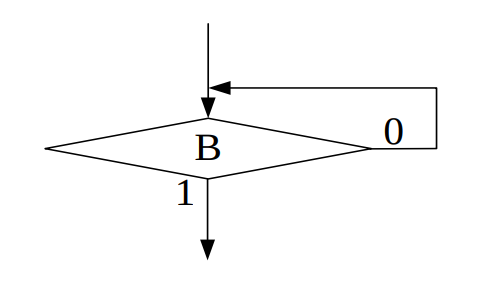
\includegraphics[width=0.3\linewidth]{delay-node}
	\caption{Ждущая вершина}
	\label{fig:delay-node}
\end{figure}

Начало работы автомата обеспечивает сигнал <<В>>, устанавливаемый
извне в «1» (интерпретируется как осведомительный сигнал). После этого
он сбрасывается в «0», а МПА после завершения работы снова переходит
в состояние покоя <<а1>>.
Для реализации МПА необходимо по ГСА построить таблицу состояний
и переходов автомата (Таблица \ref{tab:states}). 

\begin{table}[htbp]
	\scriptsize
		\caption{Таблица состояний}
	\begin{tabularx}\linewidth{|X|X|X|X|X|X|X|}
		%{|p{0.1\linewidth}|p{0.1\linewidth}|p{0.2\linewidth}|p{0.2\linewidth}|p{0.2\linewidth}|p{0.2\linewidth}|p{0.2\linewidth}|}
		\hline
		Текущее состояние & Код текущего состояния & Управляющие сигналы (вход. набор) & Осведомительные сигналы (условие) & Следующее состояние & Код следующего состояния & Сигналы возбуждения памяти\\ \hline
		\multicolumn{ 1}{|c|}{a1} & \multicolumn{ 1}{c|}{000} & y3, y1 & B & a2 & 001 & \heading{S1} \\ \cline{ 3- 7}
		\multicolumn{ 1}{|c|}{} & \multicolumn{ 1}{c|}{} & - - & !B & a1 & 000 & \heading{- -}\\ \hline
		\multicolumn{ 1}{|c|}{a2} & \multicolumn{ 1}{c|}{001} & y2, y4 & 1 & a3 & 010 & \heading{S2 R1} \\ \hline
		\multicolumn{ 1}{|c|}{a3} & \multicolumn{ 1}{c|}{010} & y1, y5, y6 & x1 & a5 & 100 & \heading{S3 R2} \\ \cline{ 3- 7}
		\multicolumn{ 1}{|c|}{} & \multicolumn{ 1}{c|}{} & y6 & !x1 & a4 & 011 & \heading{S1} \\ \hline
		\multicolumn{ 1}{|c|}{a4} & \multicolumn{ 1}{c|}{011} & -- & x3 & a2 & 001 & \heading{R2} \\ \cline{ 3- 7}
		\multicolumn{ 1}{|c|}{} & \multicolumn{ 1}{c|}{} & -- & !x3 & a5 & 100 & \heading{S3 R2 R1}\\ \hline
		\multicolumn{ 1}{|c|}{a5} & \multicolumn{ 1}{c|}{100} & y3, y5 & x2 & a1 & 000 & \heading{R3} \\ \cline{ 3- 7}
		\multicolumn{ 1}{|c|}{} & \multicolumn{ 1}{c|}{} & -- & !x2 & a1 & 000 & \heading{R3} \\ \hline
	\end{tabularx}

	\label{tab:states}
\end{table}


В таблице отмечаются состояния МПА, управляющие сигналы, формируемые в каждом состоянии при наличии определенных значений осведомительных сигналов. Кроме того, в правой колонке таблицы записываются сигналы возбуждения памяти, формируемые по кодам состояния текущего и следующего состояния памяти.

 Значения сигналов определяются таблицами переключения триггеров, выбранных для построения памяти. В данном случае память реализована на RS-триггерах.
Таблица позволяет описать логическую организацию схем КС1 и КС2,
т.е. произвести их абстрактный синтез.

\underline{Для КС1}
\begin{align*}
	y_1 &= a_3x_1+a_1B \\
	y_2 & =a_2\\
	y_3 & =a_1B+ a_5x_2\\
	y_4 &=a_2\\
	y_5 & =a_3x_1+a_5x_2\\
	y_6 & = a_3
\end{align*}

%\newpage
\underline{Для КС2}
\begin{align*}
	S_1 &=a_1B+a_3\bar{x_1} &R_1& =a_2+a_4\bar{x_3} \\
	S_2 & =a_2 	& R_2 & = a_3x_1+a_4\\
	S_3 & = a_3x_1+a_4\bar{x_3} & R_3 & = a_5
\end{align*}
	
	По полученным логическим выражениям произведем структурный синтез схем КС1 и КС2 и построим электрическую функциональную схему МПА.
	
	
	Приведем схему МПА, построенного на основе автомата Мили адресацией (Рисунок \ref{fig:mili-scheme}).
	% TODO: \usepackage{graphicx} required
	\begin{figure}[h!]
		\centering
		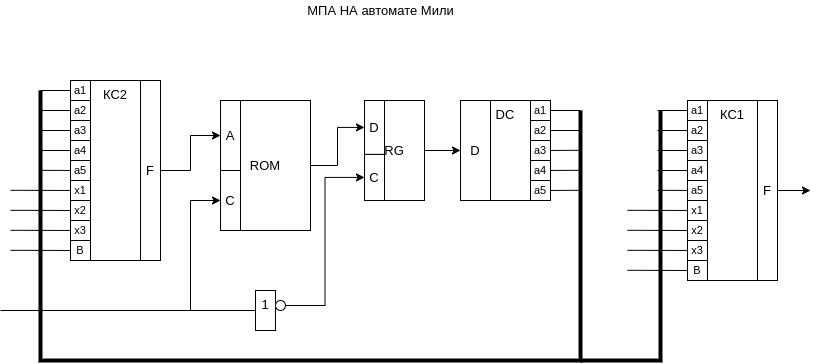
\includegraphics[width=0.8\linewidth]{mili-scheme}
		\caption{МПА на основе автомата Мили}
		\label{fig:mili-scheme}
	\end{figure}
	
	
	\newpage
	\paragraph{Реализация блока управления на базе МПА с программируемой логикой.}
	В МПА с программируемой логикой ГСА реализуется посредством микропрограммы (МКП), хранимой в управляющей памяти. Микропрограмма состоит из микрокоманд (МК), последовательность которых описывает графсхему алгоритма управления. Микрокоманда представляет собой машинное
	слово, состоящее из двух полей (Рисунок \ref{fig:op}). 
	
	% TODO: \usepackage{graphicx} required
	\begin{figure}[h!]
		\centering
		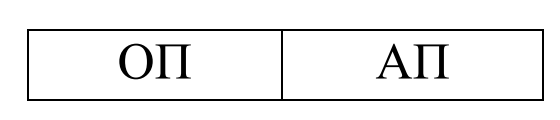
\includegraphics[width=0.3\linewidth]{op}
		\caption{Машинное слово МПА	}
		\label{fig:op}
	\end{figure}

В ОП микрокоманды записываются управляющие сигналы или их коды. В АП~---~коды номеров условных вершин
ГСА и адрес или адреса перехода к следующей микрокоманде.

Организуем ОП смешанным горизонтально-вертикальным способом. В нашем случае ОП будет состоять из трех сегментов $NY1 – NY3$, по которым распределяются управляющие сигналы (см. Таблицу \ref{tab:op-mix}).

\begin{table}[h!]
		\caption{Организация ОП смешанным способом}
	\centering
		\begin{tabular}{|c|c|c|c|c|c|}
		\hline
		\multicolumn{2}{|c|}{NY1} &  \multicolumn{2}{c|}{NY2} & \multicolumn{2}{c|}{NY3}  \\
		\hline
		\textbf{01} & y1 & \textbf{01} & y6 & \textbf{1} & y5 \\
		\hline
		\textbf{10} & y4 & \textbf{10} & y2 & \textbf{0} & отс. \\
		\hline
		\textbf{11} & yк & \textbf{11} & y3  &  &  \\
		\hline
		\textbf{00} & отс. & \textbf{00} & отс. &  &  \\
		\hline
	\end{tabular}

	\label{tab:op-mix}
\end{table}




Способы перехода в микропрограммах к следующей микрокоманде определяются форматами адресных полей МК и правилами перехода. Принудительный переход выполняется по адресу, указанному в самой МК. Это соответствует безусловному переходу команд БП. При естественной адресации микрокоманд следующая микрокоманда адресуется посредством инкремента счетчика адреса микрокоманд (СЧАМК).

\paragraph{Микропрограммный автомат с принудительной адресацией МК}
Форматы МК с двумя адресными полями при принудительной адресации
могут иметь следующий вид (Рисунок \ref{fig:mk-mix}).

% TODO: \usepackage{graphicx} required
\begin{figure}[h!]
	\centering
	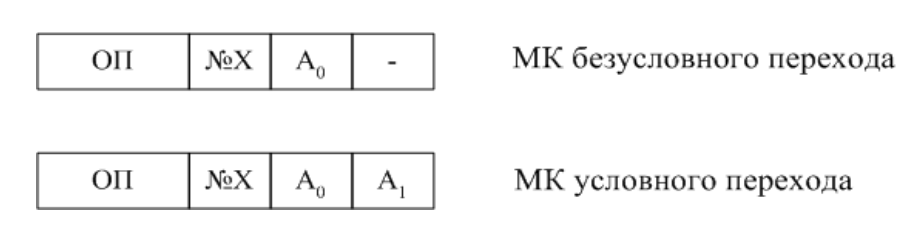
\includegraphics[width=0.5\linewidth]{mk-mix}
	\caption{Форматы микрокоманд. Принудительная адресация}
	\label{fig:mk-mix}
\end{figure}

В Таблице \ref{tab:manage-algorithm} представлена МКП, описывающая рассматриваемый алгоритм управления

\begin{table}[htbp]
		\centering
		\caption{Алгоритм управления. Принудительная адресация }
	\begin{tabular}{|c|c|c|c|c|c|c|l|}

		\hline
		Разряды & 0:1 & 2:3 & 4 & 5:6 & 7:9 & 10:12 & Прим. \\ \hline
		Адрес в УП & NY1 & NY2 & NY3 & NX & A0 & A1 & УП \\ \hline
		1 & <y1> & <y3> & - & 00 & 2 & - & БУ \\ \hline
		2 & <y4> & <y2> & - & NX1 & 3 & 4 & УП \\ \hline
		3 & - & <y6> & - & NX3 & 5 & 2 & УП \\ \hline
		4 & <y1> & <y6> & <y5> & NX2 & 7 & 6 & УП \\ \hline
		5 & - & - & - & NX2 & 7 & 6 & УП \\ \hline
		6 & - & <y3> & <y5> & 00 & 7 & - & БУ \\ \hline
		7 & <yк> & - & - & - & - & - &  -\\ \hline
	\end{tabular}

	\label{tab:manage-algorithm}
\end{table}




Опишем структуру блока формирования сигналов перехода в виде следующей
микрокоманды:
\begin{align*}
	Z_1 & = БП + \left(NX1\bar{x_1}+NX2\bar{x_2}+NX3\bar{x_3}\right) \\
	Z_2 & = NX1x1+NX2x_2+NX3x_3
\end{align*}


Приведем схему МПА с принудительной адресацией (Рисунок \ref{fig:straight-scheme}).
% TODO: \usepackage{graphicx} required
\begin{figure}[h!]
	\centering
	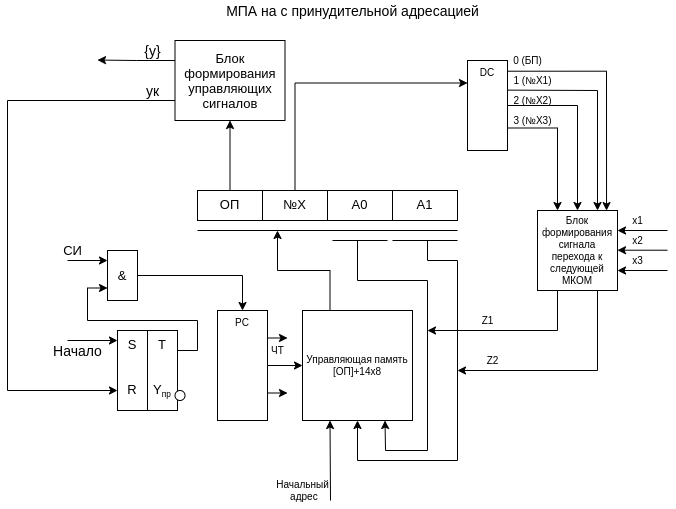
\includegraphics[width=0.7\linewidth]{straight-scheme}
	\caption{МПА с принудительной адресацией}
	\label{fig:straight-scheme}
\end{figure}


\newpage
\paragraph{Микропрограммный автомат с естественной адресацией}
Рассмотрим вариант, предлагающий наличие двух типов микрокоманд: операционной, которая выполняет полезную работу и обрабатывает операторные
вершины ГСА, и управляющей МК условного и безусловного переходов (Рисунок \ref{fig:mk-mix-nat}).

% TODO: \usepackage{graphicx} required
\begin{figure}[h!]
	\centering
	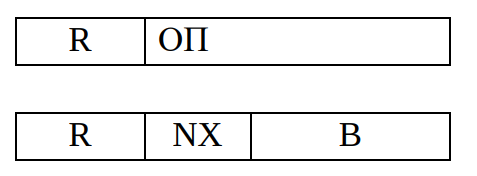
\includegraphics[width=0.4\linewidth]{mk-mix-nat}
	\caption{Формат микрокоманд. Естественная адресация}
	\label{fig:mk-mix-nat}
\end{figure}


В Таблице \ref{tab:manage-algorithm2} представлена МКП, описывающая рассматриваемый алгоритм управления. 

\begin{table}[htbp]
	\centering
				\caption{Алгоритм управления. Естественная адресация }
	\begin{tabular}{|c|c|c|c|c|c|}

		\hline
		Адр. МКОП & R & NY1 & NY2 & NY3 & доп \\ \hline
		Разр. & 0 & 1:2 & 3:4 & 5 & 6 \\ \hline
		Адр. МКОП & R & NX & B &  &  \\ \hline
		Разр. & 0 & 1:2 & \multicolumn{ 3}{c|}{3:6} \\ \hline
		1 & 0 & <y1> & <y3> & - & 0 \\ \hline
		2 & 0 & <y4> & <y2> & - & 0 \\ \hline
		3 & 1 & NX1 &  \multicolumn{ 3}{c|}{7}  \\ \hline
		4 & - & - & {<y6>}& - & 0 \\ \hline
		5 & 1 & NX3 &  \multicolumn{ 3}{c|}{2}  \\ \hline
		6 & 1 & 00 & \multicolumn{ 3}{c|}{8}  \\ \hline
		%7 & 0 & <yк> & \multicolumn{ 3}{c|}{-} \\ \hline
		7 & 0 & <y1> & <y6> & <y5> & 0 \\ \hline
		8 & 1 & NX2 &  \multicolumn{ 3}{c|}{10} \\ \hline
		9 & 0 & <yк> & -& -& 0 \\ \hline
		10 & 0 & - & <y3> & <y5> & 0 \\ \hline
		11 & 0 & <yк> & - & - & 0 \\ \hline
	\end{tabular}

	\label{tab:manage-algorithm2}
\end{table}





Опишем структуру блока формирования сигналов перехода в виде следующей
микрокоманды:
\begin{align*}
	Z_1 & =R + \bar{R}\left(NX1\bar{x_1}+NX2\bar{x_2}+NX3\bar{x_3}\right) \\
	Z_2 & = R\left[БП + \left(NX1x_1+NX2x_2+NX3x_3\right)\right]
\end{align*}

Приведем схему МПА с естественной адресацией (Рисунок \ref{fig:nature-scheme}).
% TODO: \usepackage{graphicx} required
\begin{figure}[htpb]
	\centering
	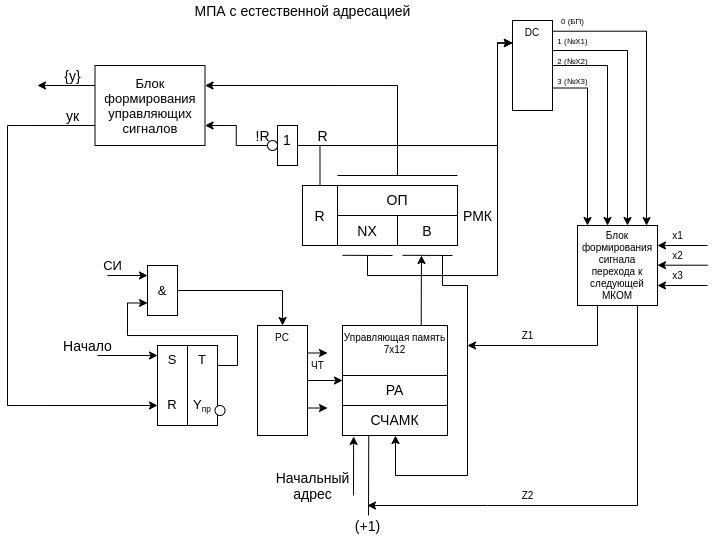
\includegraphics[width=0.8\linewidth]{nature-scheme}
	\caption{МПА с естественной адресацией}
	\label{fig:nature-scheme}
\end{figure}
%\newpage
%\vspace{42ex}
	\paragraph{Вывод:}
	В ходе данной практической работы мы ознакомились, разработали три МПА Мили на жесткой логике, УАПЛ с принудительной адресацией с двумя адресными полями, УАПЛ с естественной адресацией.
	Полученные знания применили на практике.
	
	
\end{document}

